\documentclass[letterpaper,10pt]{article}

%\setlength{\parindent}{0in}
%\usepackage{fullpage} 
\usepackage{amsmath}
\usepackage{amssymb}
\usepackage{enumerate}
\usepackage{graphicx}
\usepackage[table]{xcolor}
\usepackage{dcolumn}
\oddsidemargin 0.0in
\textwidth 6.5in
\newcolumntype{.}{D{.}{.}{-1}}
\newcommand*{\myalign}[2]{\multicolumn{1}{#1}{#2}}

%opening
\title{Final Exam}
\author{Steve Mazza}
%\date{December 9, 2011}

\begin{document}
\maketitle

\begin{description}
\item[Question 1:]
Given the differential equation $\dfrac{d^4y}{dx^4}+\dfrac{d^2y}{dx^2}=0\equiv y''''+Ay''$ derive the equivalent system of first-order ordinary differential equations.  This is a fourth order differential equation.  What order is the system of equations?  Is the system linear or nonlinear?  What does such a system of first-order ordinary differential equations represent?

%TODO: Answer question. (mazzas) Fri Jun 13 18:20:42 2014
% Based on slide deck 2, slide 7, I assume this is a linear system since it can be broken up into parts.

\item[Question 2:]
The Maxwell-Bloch equations are a sophisticated model for a laser and describe the dynamics of the electric field $E$, the mean polarization of the atoms $P$, and the population inversion $D$:
\begin{align*}
\dot{E} &= (P-E) \\
\dot{P} &= \gamma_1(ED-P) \\
\dot{D} &= \gamma_2(\lambda+1-D-EP)
\end{align*}
where $\gamma_1$ and $\gamma_2$ are decay rates of the atomic polarization and population inversion, respectively, and $\lambda$ is a pumping energy parameter.  The parameter $\lambda$ may be positive, negative, or zero; all other parameters are positive.  In the simplest case, $P$ and $D$ relax rapidly to steady values, and hence may be eliminated as follows.
\begin{enumerate}
\item Assuming $\dot{D}\approx 0$\ $\dot{P}\approx 0$, express $P$ and $D$ in terms of $E$, and thereby derive a first-order equation for the evolution of $E$.
\item Find all the fixed points of $E$.
\item Draw the bifurcation diagram of $E^*$ versus $\lambda$.  Distinguish between stable and unstable branches.
\end{enumerate}

%TODO: Answer question. (mazzas) Fri Jun 13 18:21:02 2014
% Slide deck 4, slides 31 \& 39 talks about fixed points.
% This is Strogatz problem 3.3.2, page 82.

\item[Question 3:]
What is this an example of?  What features are represented?
\begin{center}
  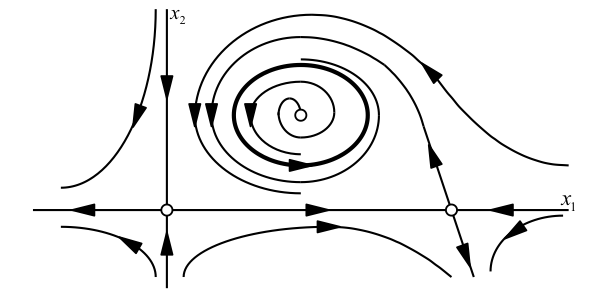
\includegraphics[scale=0.65]{images/phaseportrait.png}
\end{center}

This is a phase portrait.

From our class notes where this image was taken, ``A phase portrait is a qualitative picture of the behavior of a system in phase space.  Typically it shows fixed points, the stability of fixed points, closed orbits, and trajectories near the fixed points and closed orbits.  The phase portrait above is illustrative only and does not represent a specific system.''

Fixed points on this diagram are represented by the hollow dots. There are three; one appears at the intersection of the axes, one appears at the zero on the $x-$axis, and the third is located at the center of the sync of the closed orbit.  The closed orbit, located near the center of the diagram, is represented by the heavier closed line with the counter-clockwise directional arrow.

There are trajectories located near the fixed points which indicate stability or instability.  Trajectories moving toward fixed points indicate stability.  Trajectories moving away from fixed points indicate instability.  As seen in our diagram, a fixed point may be stable in one direction and instable in another.  A geometric representation of this would be a saddle point.  The unstable fixed point inside the closed orbit could be geometrically represented as a hill of bump in the
landcape.

\item[Question 4:]
For the Lorenz equations
\begin{align*}
\dot{x} &= \sigma(y-x) \\
\dot{y} &= rx-y-xz \\
\dot{z} &= xy-bz
\end{align*}
with $\sigma=10, r=28$, and $b=2.66666$, and initial condition $x=1.0+\delta, y=1.0$, and $z=10$, determine how long it takes the absolute error between the ``true $x$ solution'' $(\delta=0)$ to grow from $\delta$ to 0.1. Calculate for $\delta$ values of 0.01, $10^{-4}, 10^{-6}, 10^{-8}$, and $10^{-10}$.  What does this tell you about the predictability versus measurement error?  Can you estimate the Liapunov exponent? (Strogatz, 366)

%TODO: Answer question. (mazzas) Fri Jun 13 18:21:38 2014
% Slide deck 4, slide 45 talks about Liapunov exponents.
% This looks just like Strogatz, page 339.

\item[Question 5:]
Consider the iterated map given by
\[x_{n+1} = \left\{
  \begin{array}{lr}
    rx_n &  0\le x_n \le 0.5 \\
    f(1-x_n) &  0.5\le x_n \le 1
  \end{array}
\right.
\]
where $0<r<2$.  What properties do you expect to see in the orbit diagram?  Is there any condition that might cause different behavior?  The Liapunov exponent is $\lambda=\mbox{ln\ }r$. (Strogatz, 366)  What does this tell you about the behavior?

%TODO: Answer question. (mazzas) Fri Jun 13 18:21:59 2014

\item[Question 6:]
  In your own words and using no more than one paragraph, describe the difference between complex and complicated systems.  That is, in your own opinion what distinguishes the two?

  The difference between complexity and complicated systems hinges on the interactions of the parts of the system and on how difficult those interactions make predicting the future state of the system.  Emergent properties, a hallmark of complex systems, come from these highly affective interactions.  Note that systems with many moving parts and even possibly many interactions but whose outcomes are highly deterministic are not complex, but complicated.  The classic example of
  this is a watch.  Lastly, complex systems exhibit a robustness that merely complicated systems do not have.  That is, they will continue to function despite the loss of a (small) subset of its parts.

\item[Question 7:]
How are fractals and complexity related?

According to Mitchell (page 103, ``Complexity as Fractal Dimension''), the fractal dimension of an object is a measure of its complexity.  A fractal dimension is often a ratio (non-integer) that is a statistical index of complexity indicating how detail changes with scale.  This is also referred to as the Hausdorf dimension and quantifies the number of self-similar copies at each level of magnification.

\item[Question 8:]
Define what an adaptive agent-based model is and briefly describe its characteristics.

Agent based models.
\begin{itemize}
  \item Ideas drive the development of tools (quarks drive accelerators) or tools may drive the development of ideas (microscopes drive microbiology).
  \item Agent-based models are computer models that permit the exploration of complex systems in more detail.
  \item Agent-based models consist of entities of various types (the agents) endowed with limited memory and cognitive ability that are embedded in a network (connected to other agents) and whose behaviors are interdependent (usually locally).
  \item Agents follow rules.  The rules may be simple and fixed or complicated and adaptive.
  \item Adaptive agents follow metarules, which are rules about how rules can be changed.
  \item Agents often take discrete actions such as changing location, switching strategy (cooperation vs. defection), or joining or exiting a particular activity.
  \item Rules are often threshold-based, that is, rules in which the agent’s behavior remains the same until some threshold is met.
  \item Threshold effects can cause positive (more of the same) or negative (less of the same) feedbacks.
  \item Agent-based systems often exhibit complex, emergent behavior.
\end{itemize}

%TODO: Answer question. (mazzas) Fri Jun 13 18:22:45 2014
% Slide deck 1, slide 84.

\item[Question 9:]
In an engineering system consisting of various parts and mechanisms, what kinds of diversity are most applicable to determining complexity?  How might that diversity be measured?

Complexity (from slide 62)
\begin{itemize}
  \item Variation within a type seldom results in complexity
  \item Differences between types is often associated with complexity
  \item Diversity in composition is often associated with complexity
\end{itemize}

Five kinds of diversity measures (from slide 59)
\begin{itemize}
  \item Variation measures
  \item Entropy measures
  \item Distance measures
  \item Attribute measures
  \item Disjoint population measures
\end{itemize}
Also see slides 60 \& 61

%TODO: Answer question. (mazzas) Fri Jun 13 18:22:57 2014
% Slide deck 1, slides 58-62, focusing on slide 62.

\item[Question 10:]
What approaches are likely to [be] part of any attempt to harness complexity in an inherently complex system?

Traditional approaches to control (command and control) fail for complex systems.  Complex systems, however, can be harnessed by considering the primary characteristics of interdependence, connectedness, diversity, and adaptivity.  One way to harness complexity is to adjust diversity, which determines the level of exploitation or exploration.  Increasing diversity moves the system away from exploitation toward exploration.  To a point, increasing diversity helps prevent errors
(Linus' Law).

Watch for outliers in a population.  It does not take many vocal people to sway the conditions of a complex system.  Be wary of spending too much effort chasing small gains in efficiency and always leave room in the system so that failure does not cascade (as in recent bank failures).

Adjusting the interactions to remove unnecessary connections in favor of synergistic ones is another strategy.  Incentives may not support your desired outcomes.  In hierarchical structures, severing connections to parent organizations increases diversity and exploration.

Additionally, in ``Harnessing Complexity,'' Axelrod \& Cohen present a framework for harnessing complexity, which the refer to as the Complex Adaptive Systems approach.  They describe various techniques of variation, interaction, and selection that the user of a system can leverage to affect or sway the outcome of a complex adaptive system.

The following ideas are summarized from the section titled, ``What a User of the Framework Can Do,'' in the \emph{Conclusion} of their book.

\begin{description}
  \item[Variation] \ \\
    \begin{itemize}
      \item Arrange organizational routines to generate a good balance between exploration and exploitation.
      \item Link processes that generate extreme variation to processes that select with few mistakes in the attribution of credit.
    \end{itemize}
  \item[Interaction] \ \\
    \begin{itemize}
      \item Build networks of reciprocal interaction that foster trust and cooperation.
      \item Assess strategies in light of how their consequences can spread.
      \item Promote effective neighborhoods.
      \item Do not sow large failures when reaping small efficiencies.
    \end{itemize}
  \item[Selection] \ \\
    \begin{itemize}
      \item Use social activity to promote the growth and spread of valued criteria.
      \item Look for shorter-term, finer-grained measures of success that can usefully stand in for longer-run, broader goals.
    \end{itemize}
\end{description}

Detailed explanations of these approaches can be found on pages 155 -- 158.

\end{description}
\end{document}
